\documentclass[12pt,a4paper,xcolor=table]{report}
\usepackage[table,xcdraw]{xcolor}
\usepackage{geometry}
 \geometry{
 a4paper,
 left=20mm,
 top=20mm,
 right=20mm,
 bottom=20mm
 }
\usepackage[english]{babel}
% To change the name of Appendix to Annex
% \addto{\captionsenglish}{\renewcommand*{\appendixname}{Annex}}
\usepackage[utf8]{inputenc}
% Use times new roman
\usepackage{mathptmx}
\usepackage{setspace}
\usepackage[official]{eurosym}
\usepackage{textcomp}
\usepackage{pdfpages}
\usepackage{longtable}
\usepackage[compact]{titlesec}
\usepackage{graphicx}
\usepackage{fancyhdr}
\usepackage{enumitem}
\usepackage{csquotes}
\usepackage{amsmath}
\usepackage{caption}
\usepackage{subcaption}
\usepackage{float}
% ref packages
\usepackage{nameref}
% following  must be in this order
\usepackage{varioref}
\usepackage{hyperref}
\usepackage{cleveref}
\usepackage{listings}
\usepackage{xcolor}
\definecolor{codegreen}{rgb}{0,0.6,0}
\definecolor{codegray}{rgb}{0.5,0.5,0.5}
\definecolor{codepurple}{rgb}{0.58,0,0.82}
\definecolor{backcolour}{rgb}{0.95,0.95,0.92}
\lstdefinestyle{mystyle}{
    backgroundcolor=\color{backcolour},   
    commentstyle=\color{codegreen},
    keywordstyle=\color{magenta},
    numberstyle=\tiny\color{codegray},
    stringstyle=\color{codepurple},
    basicstyle=\ttfamily\footnotesize,
    breakatwhitespace=false,         
    breaklines=true,                 
    captionpos=b,                    
    keepspaces=true,                 
    numbers=left,                    
    numbersep=5pt,                  
    showspaces=false,                
    showstringspaces=false,
    showtabs=false,                  
    tabsize=2
}
\lstset{style=mystyle}
\usepackage{enumitem}
\usepackage[backend=biber,style=ieee]{biblatex}
\addbibresource{references.bib}

% % Remove chapter headings and page break
% \titleformat{\chapter}[display]
% {\normalfont\huge\bfseries}{\chaptertitlename\ \thechapter}{0pt}{\Huge}
% \titleclass{\chapter}{straight}

% % this alters "before" spacing (the second length argument) to 0
% \titlespacing*{\chapter}{0pt}{0pt}{0pt}
% \titlespacing*{\section}{0pt}{0pt}{0pt}
% \titlespacing*{\subsection}{0pt}{0pt}{0pt}

% \makeatother
% Set new lengths
\newlength{\chapheadtopskip}\setlength{\chapheadtopskip}{0pt}
\newlength{\chapheadsep}\setlength{\chapheadsep}{0pt}
\newlength{\chapheadbelowskip}\setlength{\chapheadbelowskip}{0pt}


\begin{document}
\begin{titlepage}
\begin{center}


\includegraphics[width=0.8\textwidth]{assets/ntu_logo.png}

\vspace{3cm}

{\Large CZ4042 Neural Networks}
\\[0.5cm]
{\large Assignment}

\vspace{3.5cm}

\textbf{\large Assignment 2: Object Recognition of the CIFAR-10 dataset and Text classification of Wikipage entries}

\vspace{3.5cm}


\vspace{0.5cm}

Submitted by:

\begin{table}[!htbp]
\centering
\begin{tabular}{|l|l|l|}
\hline
Eddy Lim Qing Yang & U1620115B & eddy0006@e.ntu.edu.sg \\ \hline
See Kar Teck  & U1622068J & ksee007@e.ntu.edu.sg \\ \hline
\end{tabular}
\end{table}


\vspace{1.5cm}

\vfill

% Bottom of the page
\bfseries SCHOOL OF COMPUTER SCIENCE AND ENGINEERING
\\
AY2019/2020 SEMESTER 1

\end{center}
\end{titlepage}

\pagenumbering{roman}
\tableofcontents
\listoftables
\addcontentsline{toc}{chapter}{List of Tables}
\listoffigures
\addcontentsline{toc}{chapter}{List of Figures}
\lstlistoflistings
\addcontentsline{toc}{chapter}{List of Listings}

% % \setcounter{page}{1}
\cleardoublepage
\titlespacing*{\chapter}{0pt}{0pt}{0pt}
% Set doublespace with no indent and 1em paragraph spacing

% \titleformat{\chapter}[display]
%   {\normalfont\bfseries}{}{-3em}{\Large}
% Remove gaps from list items and list heading
% \setlist[itemize]{noitemsep, topsep=-1pt}
% \doublespacing
\setlength{\parindent}{0em}
\setlength{\parskip}{1em}
\pagenumbering{arabic}
% ========================================================================
\chapter{Introduction}
In this report, 2 problems will be explored:
\begin{itemize}
    \item Classification of the Cardiotocography dataset. Experiments will be discussed in Section \ref{part1}.
    \item Regression Problem of the Graduate Admissions Predication dataset. Experiments will be discussed in Section \ref{part2}.
\end{itemize}

\section{Report overview}
\begin{itemize}
    \item In Section \ref{methods}, experimental setup and details will be discussed.
    \item In Section \ref{expt}, diagrams and data obtained from the experiments conducted will be shown.
    \item In Section \ref{conclusion}, results and answers to all queries will be discussed, along with the conclusions to the findings.
\end{itemize}

\chapter{Methods}
\label{methods}

In this chapter, the experimental setup done will be discussed.

\section{Part A: Object Recognition of the CIFAR-10 dataset}
In this problem, experiments were carried out in a google colab virtual machine (VM), using python 3.x and CPU clock of 2.3 GHz and Tesla K80 as the GPU, with 12GB gpu ram (specifications obtained from \cite{carneiro2018performance}).

The imports used in this problem is shown in Listing \ref{ls:p1}.

\begin{lstlisting}[language=Python, caption= Imports used for problem 1, label=ls:p1]
import math
import tensorflow as tf
import numpy as np
import matplotlib.pyplot as plt
import pickle
from tqdm import tqdm_notebook as tqdm
import sys
\end{lstlisting}

\section{Part B: Text classification of Wikipage entries}
Similarly in this problem, experiments were carried out in a google colab virtual machine (VM), using python 3.x and CPU clock of 2.3 GHz and Tesla K80 as the GPU, with 12GB gpu ram (specifications obtained from \cite{carneiro2018performance}).

The imports used in this problem is shown in Listing \ref{ls:p2}

\begin{lstlisting}[language=Python, caption= Imports used for problem 2, label=ls:p2]
import numpy as np
import pandas
import tensorflow as tf
import matplotlib.pyplot as plt
import csv
import time
from tqdm import tqdm_notebook as tqdm
\end{lstlisting}

\chapter{Experiment Results and conclusion}
\label{expt}
\section{Part A: Object Recognition of the CIFAR-10 dataset}
\label{part1}

The details of this dataset are as follows:
\begin{quote}
The dataset contains RGB colour images of size 32 X 32 and their labels from 0 to 9. You will be using the batch-1 of the dataset, which contains 10,000 training samples. Testing is done on 2,000 test samples. The training data and testing data are provided in files 'data\_batch\_1' and 'test\_batch\_trim' files, respectively. Sample code is given in file start\_project\_2a.py Design a convolutional neural network consisting of:

\begin{itemize}
    \item An Input layer of 3x32x32 dimensions
    \item A convolution layer $C_1$ of 50 filters of window size 9x9, VALID padding, and ReLU neurons. A max pooling layer $S_1$ with a pooling window of size 2x2, with stride = 2 and padding = 'VALID'.
    \item A convolution layer $C_2$ of 60 filters of window size 5x5, VALID padding, and ReLU neurons. A max pooling layer $S_2$ with a pooling window of size 2x2, with stride = 2 and padding = 'VALID'.
    \item A fully connected layer $F_3$ of size 300.
    \item A softmax layer $F_4$ of size 10.
\end{itemize}
\end{quote}

The definition of the cnn network as required by the question is shown in Listing \ref{ls:1_l3}, whereas the loss minimisation and accuracy prediction is shown in Listing \ref{ls:1_loss}.

\begin{lstlisting}[language=Python, caption= Definition of the cnn network, label=ls:1_l3]
def cnn(images, num_filter_1, num_filter_2, dropout=False):
    # NHWC format
    images = tf.reshape(images, [-1, IMG_SIZE, IMG_SIZE, NUM_CHANNELS])
    
    #Conv 1, 50 filters of window size 9x9, VALID padding, and ReLU
    with tf.variable_scope('CNN_Layer1'):
        conv1 = tf.layers.conv2d(
            images,
            filters=num_filter_1,
            kernel_size=[9,9],
            padding='VALID',
            activation=tf.nn.relu)
        pool1 = tf.layers.max_pooling2d(
            conv1,
            pool_size=2,
            strides=2,
            padding='VALID')
        if dropout:
            pool1 = tf.layers.dropout(pool1, 0.25)

    with tf.variable_scope('Char_CNN_Layer2'):
        conv2 = tf.layers.conv2d(
            pool1,
            filters=num_filter_2,
            kernel_size=[5,5],
            padding='VALID',
            activation=tf.nn.relu)
        pool2 = tf.layers.max_pooling2d(
            conv2,
            pool_size=2,
            strides=2,
            padding='VALID')
        if dropout:
            pool2 = tf.layers.dropout(pool2, 0.25)

    dim = pool2.get_shape()[1].value * pool2.get_shape()[2].value * pool2.get_shape()[3].value 
    pool2_ = tf.reshape(pool2, [-1, dim])
    
    # Fully connected layer size 300
    f3 = tf.layers.dense(pool2_, 300, activation=tf.nn.relu)
    if dropout:
        f3 = tf.layers.dropout(f3, 0.5)

    #Softmax, size 10. Note that softmax happens at softmax_entropy step
    f4 = tf.layers.dense(f3, NUM_CLASSES, activation=None)

    return conv1, pool1, conv2, pool2, f4
\end{lstlisting}

\begin{lstlisting}[language=Python, caption= Loss minimisation and accuracy prediction, label=ls:1_loss]
x = tf.placeholder(tf.float32, [None, IMG_SIZE*IMG_SIZE*NUM_CHANNELS])
y_ = tf.placeholder(tf.float32, [None, NUM_CLASSES])

conv_1, pool_1, conv_2, pool_2, logits = cnn(x, 50, 60)
cross_entropy = tf.nn.softmax_cross_entropy_with_logits_v2(labels=y_, logits=logits)
loss = tf.reduce_mean(cross_entropy)
train_step = tf.train.GradientDescentOptimizer(learning_rate).minimize(loss)

correct_prediction = tf.equal(tf.argmax(logits, 1), tf.argmax(y_, 1))
correct_prediction = tf.cast(correct_prediction, tf.float32)
accuracy = tf.reduce_mean(correct_prediction)
\end{lstlisting}

Additionally the handling of batches sizes are shown in Listing \ref{ls:1_batch_size}.

\begin{lstlisting}[language=Python, caption= Batch size setup, label=ls:1_batch_size]
# Handle in batches
for start, end in zip(range(0, len(train_X), batch_size), range(batch_size, len(train_X), batch_size)):
    _, batch_cost = sess.run([train_step, loss], {x: train_X[start:end], y_: train_Y[start:end]})
    train_cost_.append(batch_cost)
\end{lstlisting}

Finally, the training results used in this experiment is assumed to be the ones obtained from cross-validation obtained from Listing \ref{ls:1_folds}, while the test set used are assumed to be the test set obtained from the initial 70:30 split from the original data.

\subsection{Question 1}
\label{1q1}
\begin{quote}
Train the network by using mini-batch gradient descent learning. Set $batch size =128$, and learning rate $\alpha = 0.001$. Images should be scaled.

a. Plot the training cost and the test accuracy against learning epochs.

b. For any two test patterns, plot the feature maps at both convolution layers ($C_1$ and $C_2$) and pooling layers ($S_1$ and $S_2$) along with the test patterns.
\end{quote}

\subsubsection{Part A}
The following plot in Figure \ref{fig:1a} is obtained for Q1a.
\begin{figure}[H]
    \begin{subfigure}{1\textwidth}
        \centering
        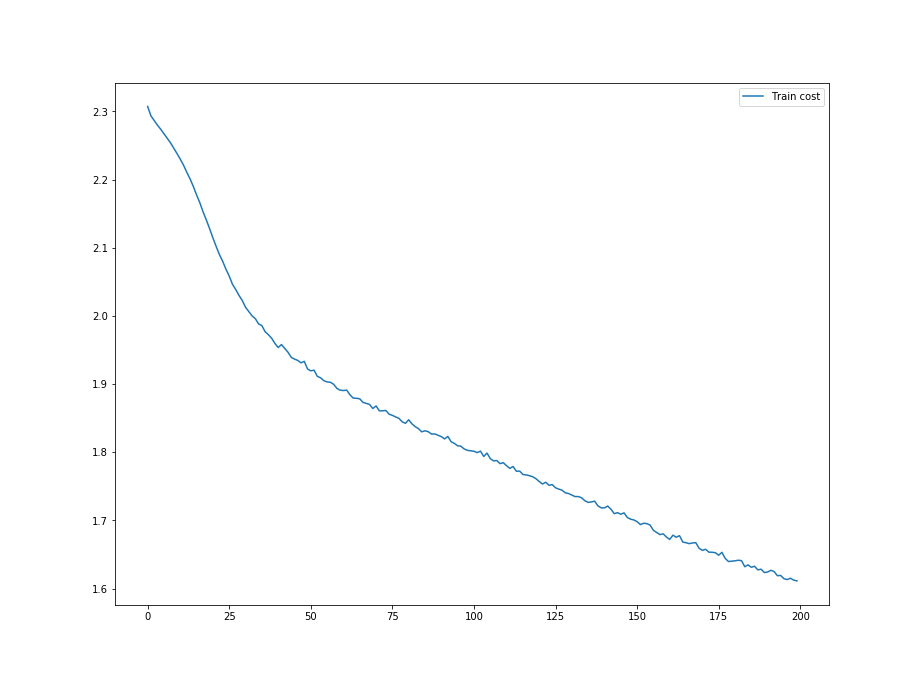
\includegraphics[width=0.8\linewidth]{assets/plots1/q1a_1.png}
        \caption{Training cost against epochs for cnn}
    \end{subfigure}
    \begin{subfigure}{1\textwidth}
        \centering
        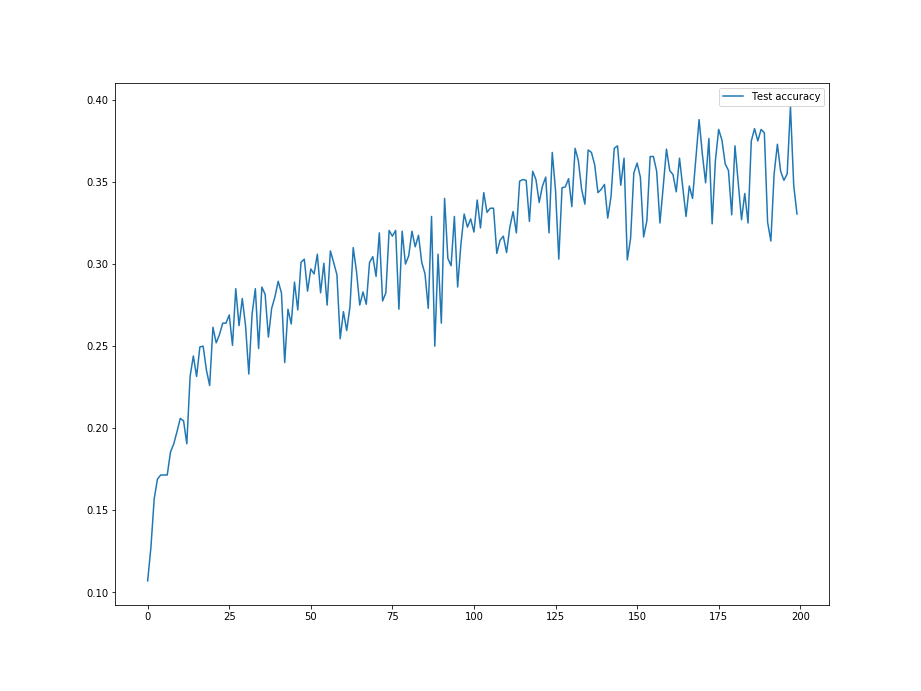
\includegraphics[width=0.8\linewidth]{assets/plots1/q1a_2.png}
        \caption{Test accuracy against epochs for cnn}
    \end{subfigure}
    \caption{Plot of training cost and testing accuracy against epochs for CNN object recognition}
    \label{fig:1a}
\end{figure}

\subsubsection{Part B}
Test Pattern 1 is shown in Figure \ref{fig:1b_1}.
\begin{figure}[H]
    \begin{subfigure}{0.5\textwidth}
        \centering
        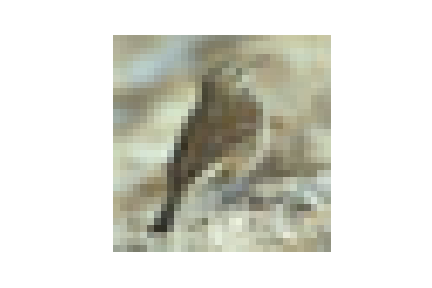
\includegraphics[width=1\linewidth]{assets/plots1/q1a_test_pattern_0.png}
        \caption{Test Pattern}
    \end{subfigure}
    \begin{subfigure}{0.5\textwidth}
        \centering
        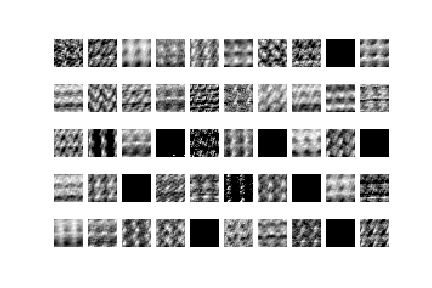
\includegraphics[width=1\linewidth]{assets/plots1/q1a_conv1_0.png}
        \caption{$\textit{C}_1$ Feature Map}
    \end{subfigure}
    \begin{subfigure}{0.5\textwidth}
        \centering
        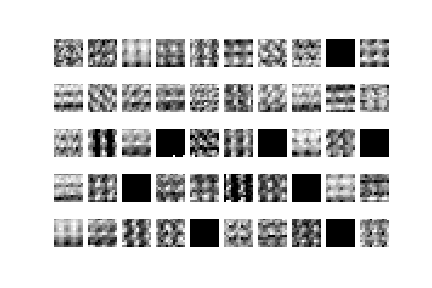
\includegraphics[width=1\linewidth]{assets/plots1/q1a_pool1_0.png}
        \caption{$\textit{S}_1$ Feature Map}
    \end{subfigure}
    \begin{subfigure}{0.5\textwidth}
        \centering
        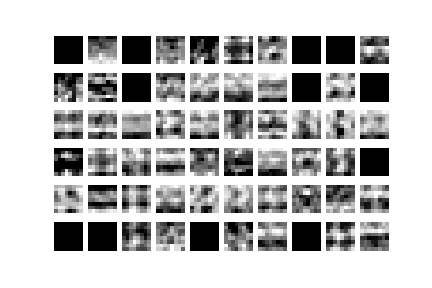
\includegraphics[width=1\linewidth]{assets/plots1/q1a_conv2_0.png}
        \caption{$\textit{C}_2$ Feature Map}
    \end{subfigure}
    \begin{subfigure}{0.5\textwidth}
        \centering
        
\includegraphics[width=1\linewidth]{assets/plots1/q1a_pool2_0.png}
        \caption{$\textit{S}_2$ Feature Map}
    \end{subfigure}
    \caption{Feature maps of test pattern 1}
    \label{fig:1b_1}
\end{figure}

Test Pattern 2 is shown in Figure \ref{fig:1b_2}.
\begin{figure}[H]
    \begin{subfigure}{0.5\textwidth}
        \centering
        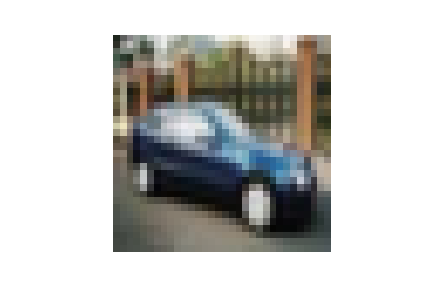
\includegraphics[width=1\linewidth]{assets/plots1/q1a_test_pattern_1.png}
        \caption{Test Pattern}
    \end{subfigure}
    \begin{subfigure}{0.5\textwidth}
        \centering
        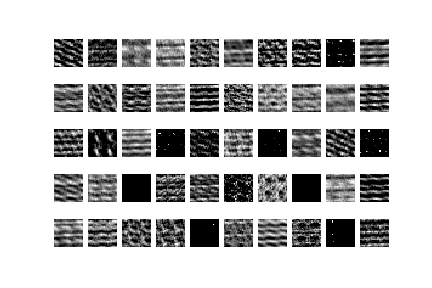
\includegraphics[width=1\linewidth]{assets/plots1/q1a_conv1_1.png}
        \caption{$\textit{C}_1$ Feature Map}
    \end{subfigure}
    \begin{subfigure}{0.5\textwidth}
        \centering
        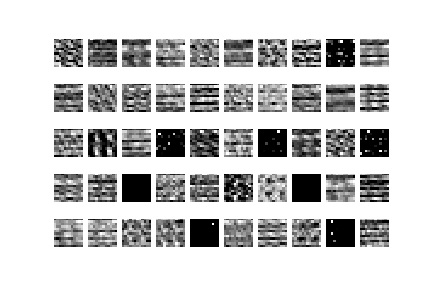
\includegraphics[width=1\linewidth]{assets/plots1/q1a_pool1_1.png}
        \caption{$\textit{S}_1$ Feature Map}
    \end{subfigure}
    \begin{subfigure}{0.5\textwidth}
        \centering
        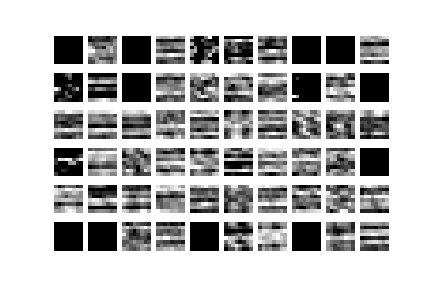
\includegraphics[width=1\linewidth]{assets/plots1/q1a_conv2_1.png}
        \caption{$\textit{C}_2$ Feature Map}
    \end{subfigure}
    \begin{subfigure}{0.5\textwidth}
        \centering
        
\includegraphics[width=1\linewidth]{assets/plots1/q1a_pool2_1.png}
        \caption{$\textit{S}_2$ Feature Map}
    \end{subfigure}
    \caption{Feature maps of test pattern 2}
    \label{fig:1b_2}
\end{figure}

\subsection{Question 2}
\label{1q2}
\begin{quote}
Using a grid search, find the optimal numbers of feature maps for part (1) at the convolution layers. Use the test accuracy to determine the optimal number of feature maps.
\end{quote}

\subsubsection{Part A}
\begin{figure}[H]
    \begin{subfigure}{0.5\textwidth}
        \centering
        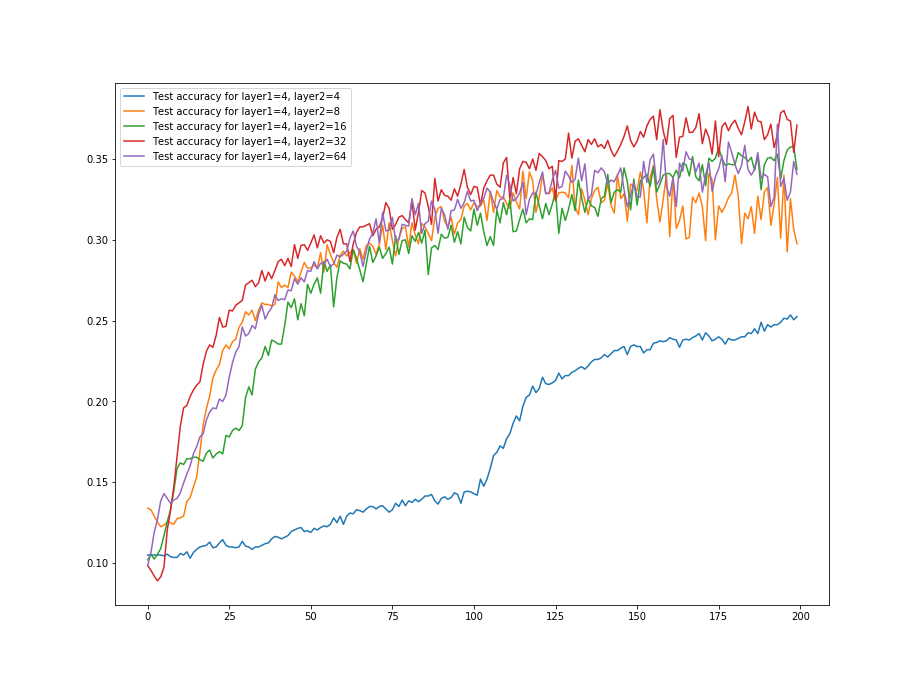
\includegraphics[width=1\linewidth]{assets/plots1/q2_0.png}
        \caption{Training cost for cnn}
    \end{subfigure}
    \begin{subfigure}{0.5\textwidth}
        \centering
        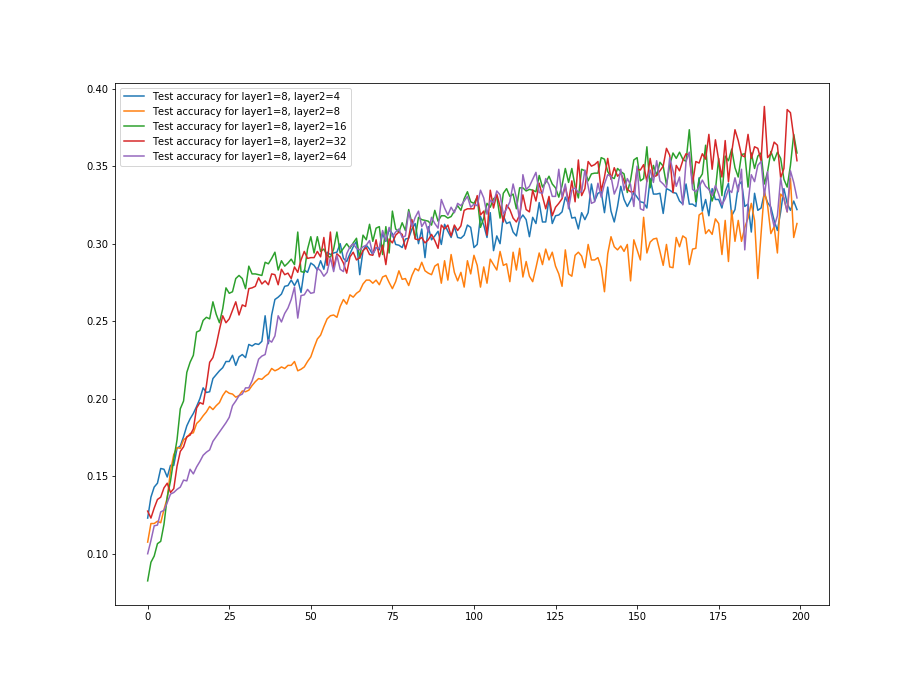
\includegraphics[width=1\linewidth]{assets/plots1/q2_1.png}
        \caption{Training cost for cnn}
    \end{subfigure}
    \begin{subfigure}{0.5\textwidth}
        \centering
        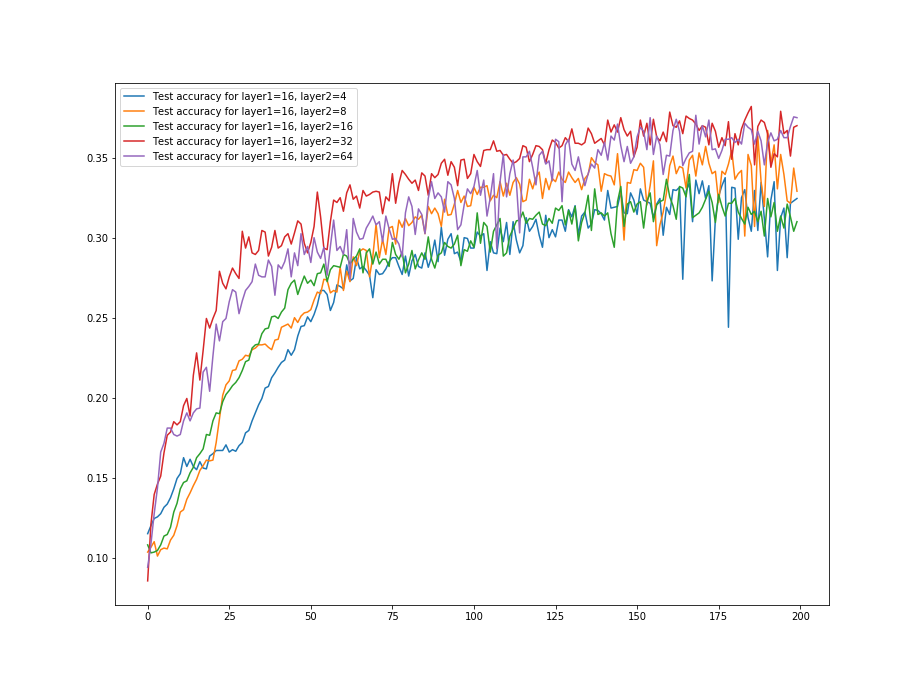
\includegraphics[width=1\linewidth]{assets/plots1/q2_2.png}
        \caption{Test accuracy for cnn}
    \end{subfigure}
    \begin{subfigure}{0.5\textwidth}
        \centering
        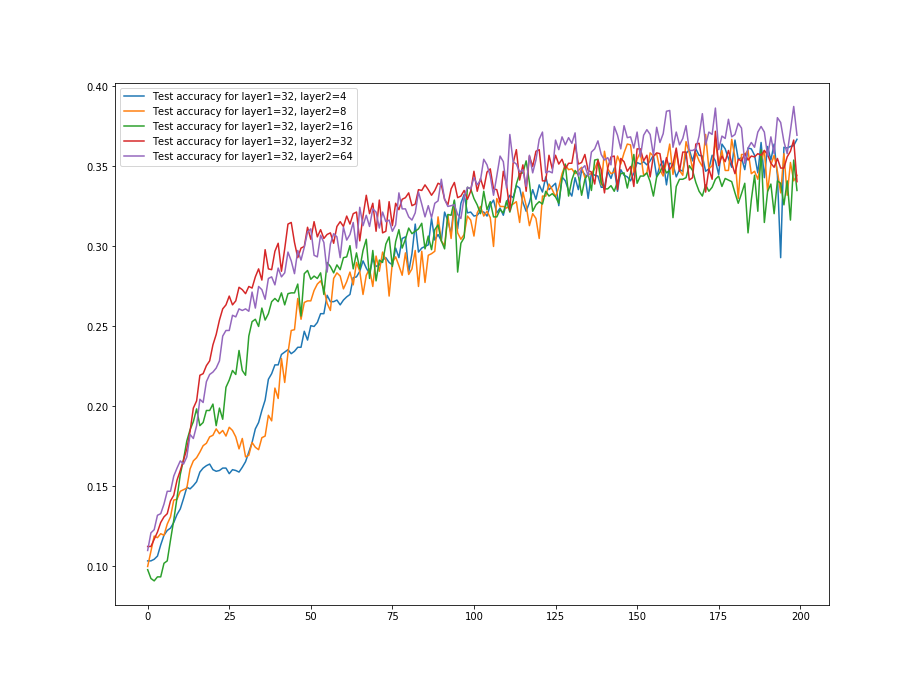
\includegraphics[width=1\linewidth]{assets/plots1/q2_3.png}
        \caption{Test accuracy for cnn}
        \label{fig:2_4}
    \end{subfigure}
    \begin{subfigure}{0.5\textwidth}
        \centering
        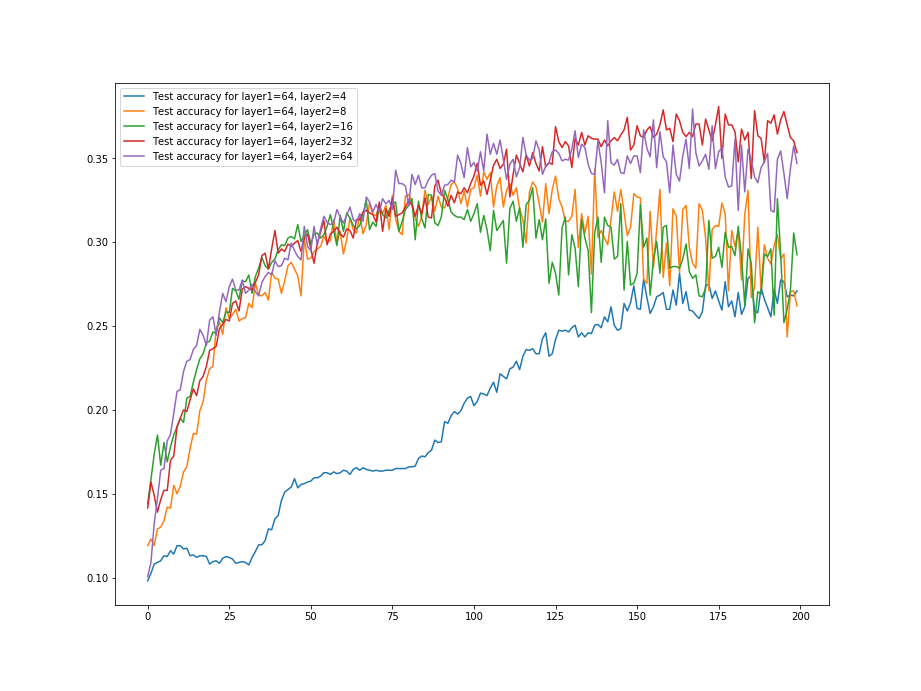
\includegraphics[width=1\linewidth]{assets/plots1/q2_4.png}
        \caption{Test accuracy for cnn}
    \end{subfigure}
    \caption{Plot of testing accuracy against epochs for different number of feature maps}
    \label{fig:2}
\end{figure}

From the results as shown in Figure \ref{fig:2_4}, having 32 feature maps in convolution layer 1 and 64 feature maps in convolution layer 2 resulted in the highest accuracy among all the others.


\subsection{Question 3}
\label{1q3}
\begin{quote}
Using the optimal number of filters found in part (2), train the network by:

a. Adding the momentum term with momentum $\gamma = 0.1$.

b. Using RMSProp algorithm for learning

c. Using Adam optimizer for learning

d. Adding dropout to the layers

Plot the training costs and test accuracies against epochs for each case.
\end{quote}

\begin{figure}[H]
    \begin{subfigure}{0.5\textwidth}
        \centering
        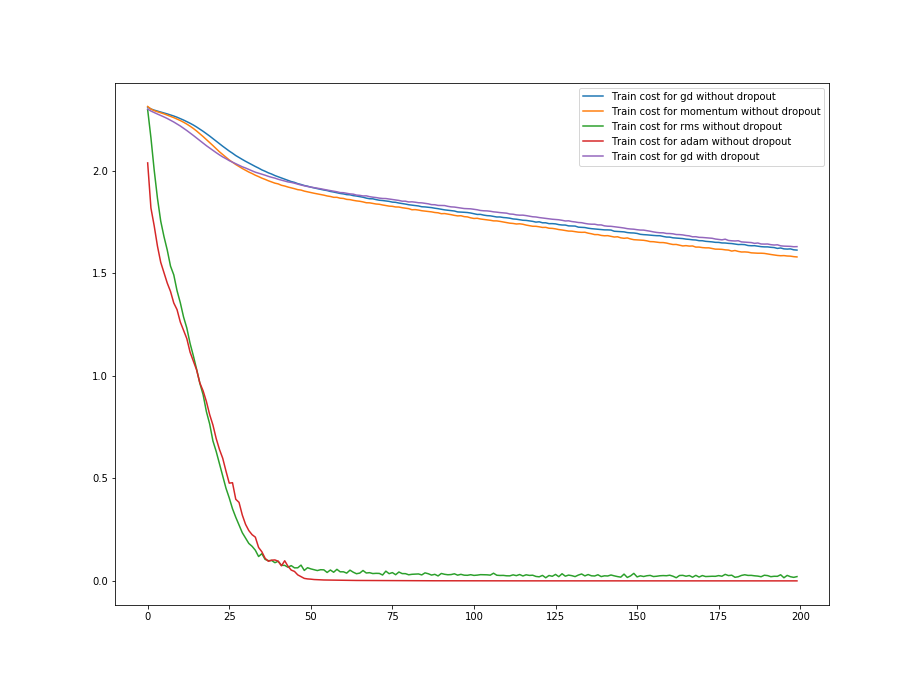
\includegraphics[width=1\linewidth]{assets/plots1/q3_1.png}
        \caption{Training cost for CNN}
        \label{fig:3_a}
    \end{subfigure}
    \begin{subfigure}{0.5\textwidth}
        \centering
        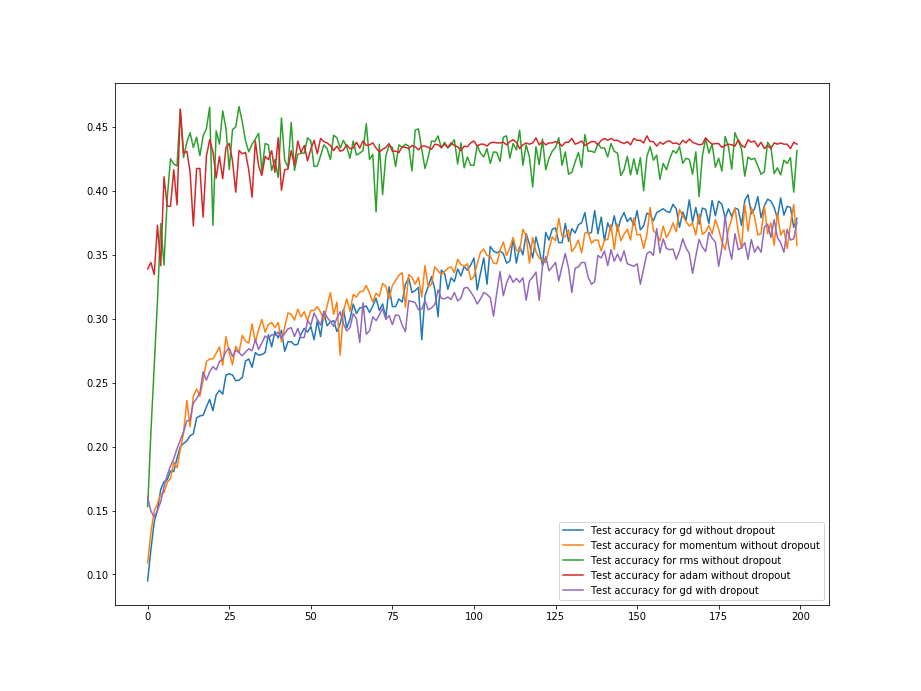
\includegraphics[width=1\linewidth]{assets/plots1/q3_2.png}
        \caption{Testing accuracy for CNN}
        \label{fig:3_b}
    \end{subfigure}
    \caption{Plot of training cost and testing accuracy against epochs for different optimizers}
    \label{fig:3}
\end{figure}

\subsection{Question 4}
\label{1q4}
\begin{quote}
Compare the accuracies of all the models from parts (1) - (3) and discuss their performances.
\end{quote}

For this experiment, we compared the performances against the original network without dropout. For network with momentum added, the accuracy is similar to the original network but its has a better learning rate as shown as the gradient being steeper. This is due to the fact that momentum causes the algorithm converges faster because oscillations are kept in one direction hence allowing a higher learning rate. Also, the RMSProp and Adam optimizers converges a lot faster in Figure \ref{fig:3_a} and has higher accuracy in Figure \ref{fig:3_a} than the other networks using other optimizers.

For the network using RMSProp, it has significantly better accuracy and performance compared to just adding momentum. It has a very high learning rate and it takes a larger step towards the minima. This is because it restricts the window of past gradients that are accumulated to be some fixed size. This ensures that learning continues to make progress even after many iterations of updates have been done. It uses an exponentially decaying average to discard the history from extreme past and this causes the algorithm to converge at a faster rate. 

The network using the Adam Optimizer has the best performance because it uses an adaptive learning rate method. Learning rates are stored for every parameter in the Adam Optimizer and it uses the squared gradients to scale the learning rate and the decaying average of the gradient instead of gradient itself. This resulted in high learning rate similar to when RMSProp is used and it has less fluctuations in the accuracy as reflected in Figure \ref{fig:3}. 
\section{Part B: Regression Problem of the Graduate Admissions Predication dataset}
\label{part2}
The details of the dataset are given as follows:
\begin{quote}
This assignment uses the data from the Graduate Admissions Predication [2]. The dataset contains several parameters, like GRE score (out of 340), TOEFL score (out of 120), university Rating (out of 5), strengths of Statement of Purpose and Letter of Recommendation (out of 5), undergraduate GPA (out of 10), research experience (either 0 or 1), that are considered important during the application for Master Programs. The predicted parameter is the chance of getting an admit (ranging from 0 to 1). You can obtain the data from: https://www.kaggle.com/mohansacharya/graduate-admissions
\end{quote}

In this problem, the dataset is divided at a 70:30 ratio for training and testing.

The neural network is defined as in Listing \ref{ls:2_nn}, with the loss and weight regularisation functions defined in Listing \ref{ls:2_cost}.

\begin{lstlisting}[language=Python, caption= Feedforward neural network (layers controlled by layers parameter), label=ls:2_nn]
def ffn(x, feature_size, neuron_size, weight_decay_beta, layers=3, dropout=False):
    """Feedforward net with hidden layers
    """
    sum_regularization = 0
    with tf.name_scope('hidden'):
        weights = tf.Variable(tf.truncated_normal([feature_size, neuron_size], stddev=1.0 / np.sqrt(feature_size), dtype=tf.float32), name='weights')
        biases = tf.Variable(tf.zeros([neuron_size]), dtype=tf.float32, name='biases')
        h  = tf.nn.relu(tf.matmul(x, weights) + biases)
        if dropout:
            h = tf.nn.dropout(h, 0.8)
        sum_regularization += weight_decay_beta * tf.nn.l2_loss(weights)
    if layers > 3:
        for i in range(layers-3):
            with tf.name_scope('hidden{}'.format(i)):
                weights = tf.Variable(tf.truncated_normal([neuron_size, neuron_size], stddev=1.0 / np.sqrt(neuron_size), dtype=tf.float32), name='weights')
                biases = tf.Variable(tf.zeros([neuron_size]), dtype=tf.float32, name='biases')
                h  = tf.nn.relu(tf.matmul(h, weights) + biases)
                if dropout:
                    h = tf.nn.dropout(h, 0.8)
                sum_regularization += weight_decay_beta * tf.nn.l2_loss(weights)
    with tf.name_scope('linear'):
        weights = tf.Variable(tf.truncated_normal([neuron_size, 1], stddev=1.0 / np.sqrt(neuron_size), dtype=tf.float32), name='weights')
        biases  = tf.Variable(tf.zeros([1]), dtype=tf.float32, name='biases')
        u = tf.matmul(h, weights) + biases
        sum_regularization += weight_decay_beta * tf.nn.l2_loss(weights)


    return u, sum_regularization
\end{lstlisting}

\begin{lstlisting}[language=Python, caption= loss and weight regularisation functions, label=ls:2_cost]
def create_model(feature_size, neuron_size, weight_decay_beta, learning_rate, layers=3, dropout=False):
    # Create the model
    x = tf.placeholder(tf.float32, [None, feature_size])
    y_ = tf.placeholder(tf.float32, [None, 1])
    y, regularizer = ffn(x, feature_size, neuron_size, weight_decay_beta, layers=layers, dropout=dropout)

    #Create the gradient descent optimizer with the given learning rate.
    optimizer = tf.train.GradientDescentOptimizer(learning_rate)
    cost = tf.square(y_ - y)
    loss = tf.reduce_mean(cost + regularizer)
    train_op = optimizer.minimize(loss)
    return y, train_op, y_, x, loss
\end{lstlisting}

Mini-batch gradient descend is done through Listing \ref{ls:mini_batch}.

\begin{lstlisting}[language=Python, caption= Mini-batch, label=ls:mini_batch]
            for start, end in zip(range(0, len(train_x), batch_size), range(batch_size, len(train_x), batch_size)):
                train_op.run(feed_dict={x: train_x[start:end], y_: train_y[start:end]})
\end{lstlisting}

\subsection{Question 1}
\label{2q1}
\begin{quote}
1. Design a 3-layer feedforward neural network consists of an input layer, a hidden-layer of 10 neurons having ReLU activation functions, and a linear output layer. Use mini-batch gradient descent with a batch size = 8, L2
regularization at weight decay parameter = $10^{-3}$ and a learning rate = $10^{-3}$ to train the network.

a) Use the train dataset to train the model and plot both the train and test errors against epochs.

b) State the approximate number of epochs where the test error is minimum and use it to stop training.

c) Plot the predicted values and target values for any 50 test samples.
\end{quote}
\subsubsection{Part A}

\begin{figure}[H]
    \centering
    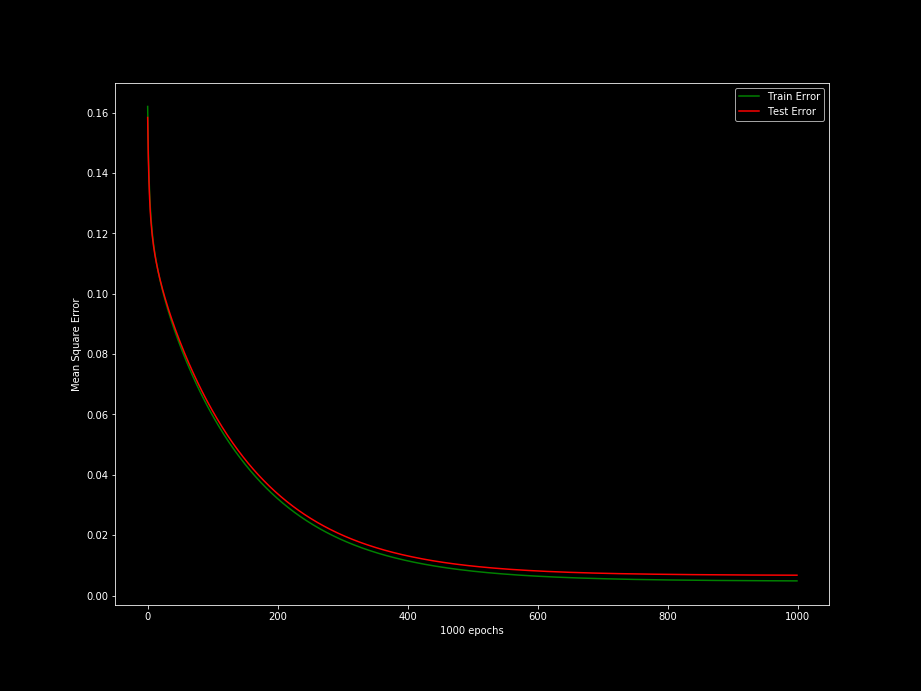
\includegraphics[width=0.8\linewidth]{assets/plots2/part2_Q1a.png}
    \caption{Plot of training and testing errors against epochs}
    \label{fig:2_1a}
\end{figure}

Figure \ref{fig:2_1a} shows the plot of training and testing errors against epochs for the 3-layer feedforward neural network as specified in the question.

\subsubsection{Part B}
Upon close inspection, it can be seen that the test error converges at around 900-1000 epochs. As such, we will use 1000 epochs as the point with minimum error.

\subsubsection{Part C}
\begin{figure}[H]
    \centering
    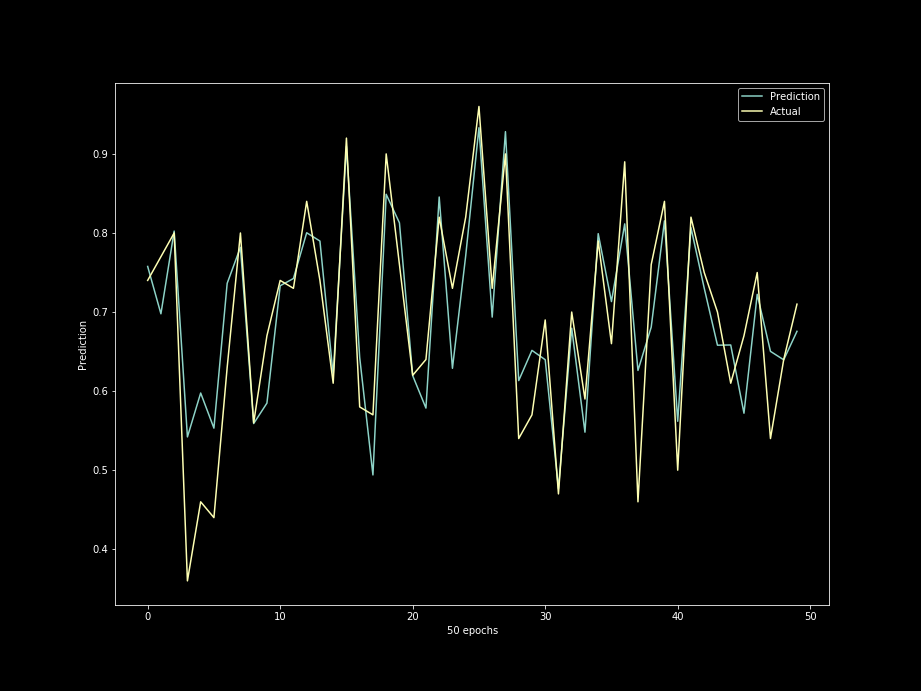
\includegraphics[width=0.8\linewidth]{assets/plots2/part2_Q1c.png}
    \caption{Plot of predicted values and target values against epochs for 50 test samples}
    \label{fig:2_1c}
\end{figure}

Figure \ref{fig:2_1c} shows the plot of predicted vs actual values. As can be seen from the plot, most predicted values are actually close to the actual values obtained. This is consistent with the low test error obtained in \ref{fig:2_1c}.

\subsection{Question 2}
\label{2q2}
\begin{quote}
2. Use the train data to compute (and plot) an 8X8 correlation matrix between the different feature scores and the corresponding chances of admit.

a) Which features are most correlated to each other? Is it justifiable?

b) What features have the highest correlations with the chances of admit?
\end{quote}
\subsubsection{Part A}

\begin{longtable}[c]{|c|c|c|c|c|c|c|c|c|}
\hline
\rowcolor[HTML]{85A4FF} 
 & \begin{tabular}[c]{@{}c@{}}GRE \\ Score\end{tabular} & \begin{tabular}[c]{@{}c@{}}TOEFL \\ Score\end{tabular} & \begin{tabular}[c]{@{}c@{}}University \\ Rating\end{tabular} & SOP & LOR & CGPA & Research & \begin{tabular}[c]{@{}c@{}}Chance \\ of Admit\end{tabular} \\ \hline
\endfirsthead
%
\endhead
%
\cellcolor[HTML]{C0C0C0}\begin{tabular}[c]{@{}c@{}}GRE \\ Score\end{tabular} & 1.0 & 0.836 & 0.669 & 0.613 & 0.558 & 0.833 & 0.580 & 0.803 \\ \hline
\cellcolor[HTML]{C0C0C0}\begin{tabular}[c]{@{}c@{}}TOEFL \\ Score\end{tabular} & 0.836 & 1.0 & 0.696 & 0.658 & 0.568 & 0.828 & 0.490 & 0.792 \\ \hline
\cellcolor[HTML]{C0C0C0}\begin{tabular}[c]{@{}c@{}}University \\ Rating\end{tabular} & 0.669 & 0.696 & 1.0 & 0.735 & 0.660 & 0.746 & 0.448 & 0.711 \\ \hline
\cellcolor[HTML]{C0C0C0}SOP & 0.613 & 0.658 & 0.735 & 1.0 & 0.730 & 0.718 & 0.444 & 0.676 \\ \hline
\cellcolor[HTML]{C0C0C0}LOR & 0.558 & 0.568 & 0.660 & 0.730 & 1.0 & 0.670 & 0.397 & 0.670 \\ \hline
\cellcolor[HTML]{C0C0C0}CGPA & 0.833 & 0.828 & 0.746 & 0.718 & 0.670 & 1.0 & 0.522 & 0.873 \\ \hline
\cellcolor[HTML]{C0C0C0}Research & 0.580 & 0.490 & 0.448 & 0.444 & 0.397 & 0.521 & 1.0 & 0.553 \\ \hline
\cellcolor[HTML]{C0C0C0}\begin{tabular}[c]{@{}c@{}}Chance \\ of Admit\end{tabular} & 0.803 & 0.792 & 0.711 & 0.676 & 0.670 & 0.873 & 0.553 & 1.0 \\ \hline
\caption{Correlation Matrix}
\label{tab:corr_matrix}\\
\end{longtable}

Table \ref{tab:corr_matrix} shows the 8x8 correlation matrix between the different feature scores and chance to admit. The features with the highest correlation with each other are the TOEFL Score and GRE Score. The relationship between both of them may be because the GRE Test is a critical thinking and reasoning test usually conducted in English, while TOEFL is a English proficiency test. Therefore if the student score higher in TOEFL, means they might more likely understand what the GRE Test contents are which could improve their scores.

\subsubsection{Part B}
CGPA is the feature that is the most correlated to Chance of Admit, while the GRE Score is the second most correlated to Chance of Admit.

\subsection{Question 3}
\label{2q3}
\begin{quote}
3. Recursive feature elimination (RFE) is a feature selection method that removes unnecessary features from the inputs. Start by removing one input feature that causes the minimum drop (or maximum improvement) in performance. Repeat the procedure recursively on the reduced input set until the optimal number of input features is reached. Remove the features one at a time. Compare the accuracy of the model with all input features, with models using 6 input features and 5 input features selected using RFE. Comment on the observations.
\end{quote}
\subsubsection{RFE iteration 1, with 6 features}
\begin{figure}[H]
    \begin{subfigure}{1\textwidth}
        \centering
        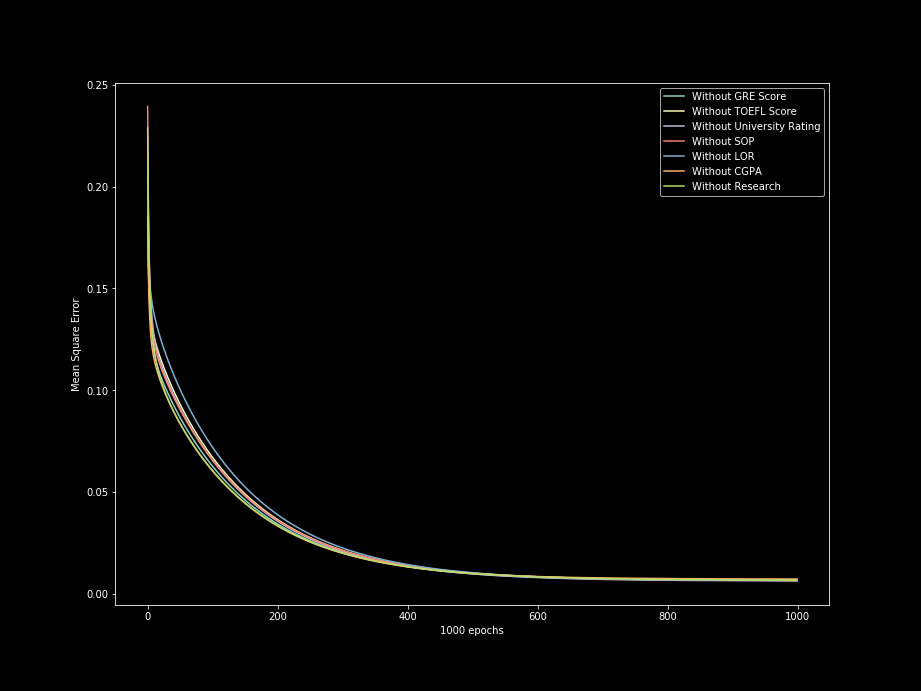
\includegraphics[width=0.8\linewidth]{assets/plots2/part3_2.png}
        \caption{Test error with RFE iteration 1}
        \label{fig:rfe1}
    \end{subfigure} 
\end{figure}
\begin{figure}[H]
    \ContinuedFloat
    \begin{subfigure}{1\textwidth}
        \centering
        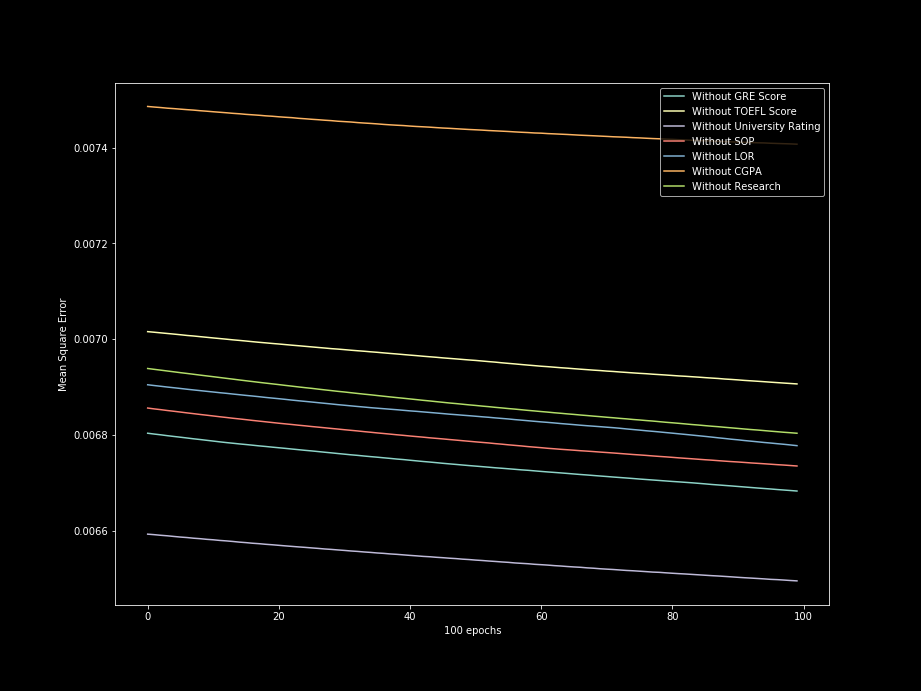
\includegraphics[width=0.8\linewidth]{assets/plots2/part3_3.png}
        \caption{Test error with RFE iteration 1 - last 100 epochs}
        \label{fig:rfe1_zoom}
    \end{subfigure}
\end{figure}

In the first iteration of RFE, it can be seen in Figure \ref{fig:rfe1_zoom} that University Ranking, followed by GRE, when removed, gives the least mean square error. This means that the removal of University Ranking will cause the least drop in performance for the model. Thus, we eliminate University Ranking in the first iteration of RFE.

\subsubsection{RFE iteration 2, with 5 features}
\begin{figure}[H]
    \begin{subfigure}{1\textwidth}
        \centering
        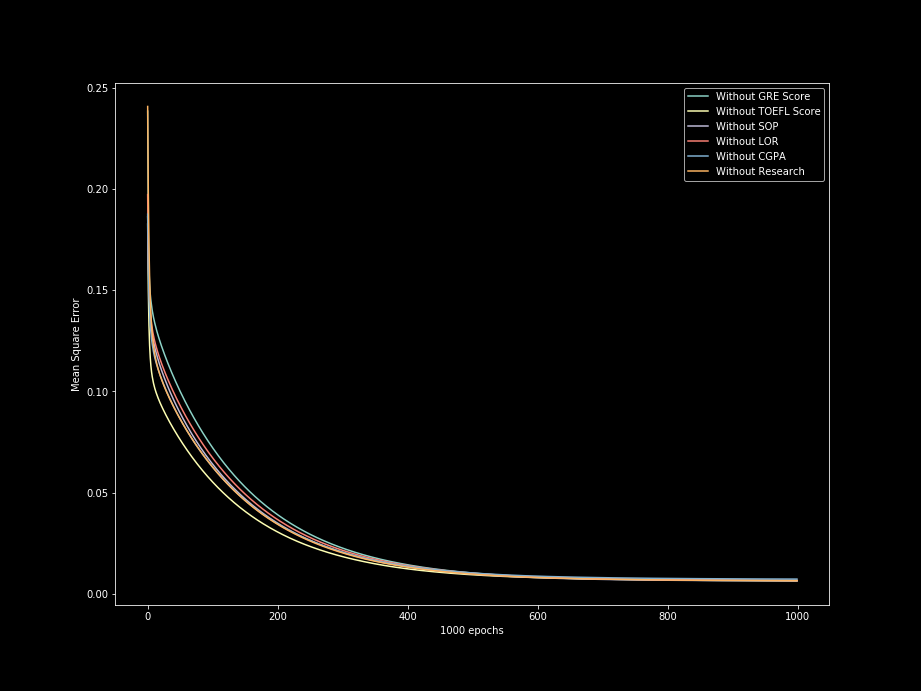
\includegraphics[width=0.8\linewidth]{assets/plots2/part3_5.png}
        \caption{Test error with RFE iteration 2}
        \label{fig:rfe2}
    \end{subfigure}
\end{figure}
\begin{figure}[H]
    \ContinuedFloat
    \begin{subfigure}{1\textwidth}
        \centering
        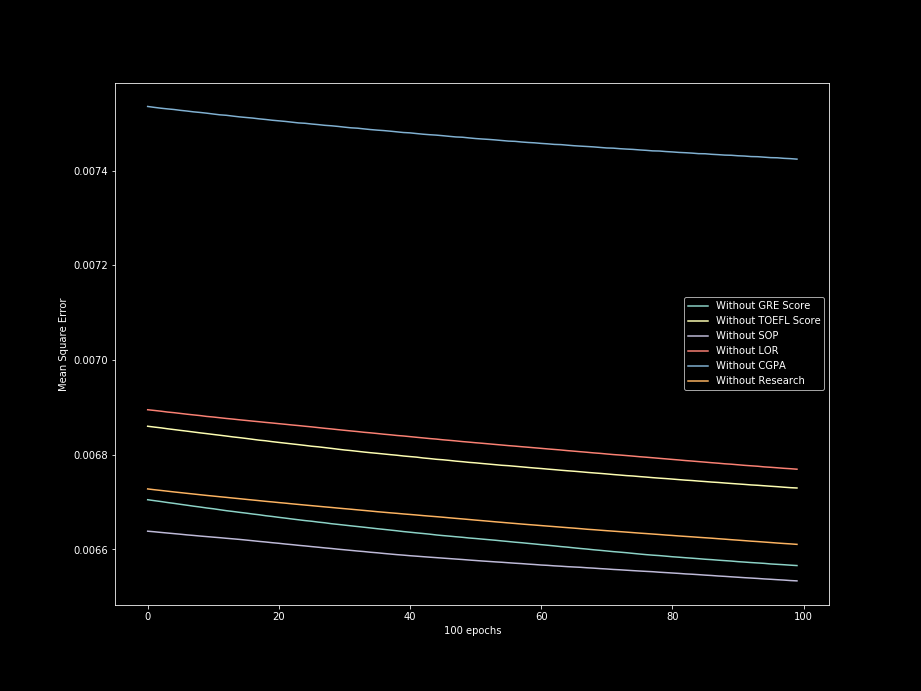
\includegraphics[width=0.8\linewidth]{assets/plots2/part3_6.png}
        \caption{Test error with RFE iteration 2 - last 100 epochs}
        \label{fig:rfe2_zoom}
    \end{subfigure}
\end{figure}

In the second iteration of RFE, it can be seen in Figure \ref{fig:rfe1_zoom} that the SOP when removed, gives the least mean square error. Similar to University Ranking, it means that the removal of SOP will cause the least drop in performance for the model. Therefore, we will remove this feature next in RFE.

\subsubsection{RFE comparisons}
\begin{figure}[H]
    \begin{subfigure}{1\textwidth}
        \centering
        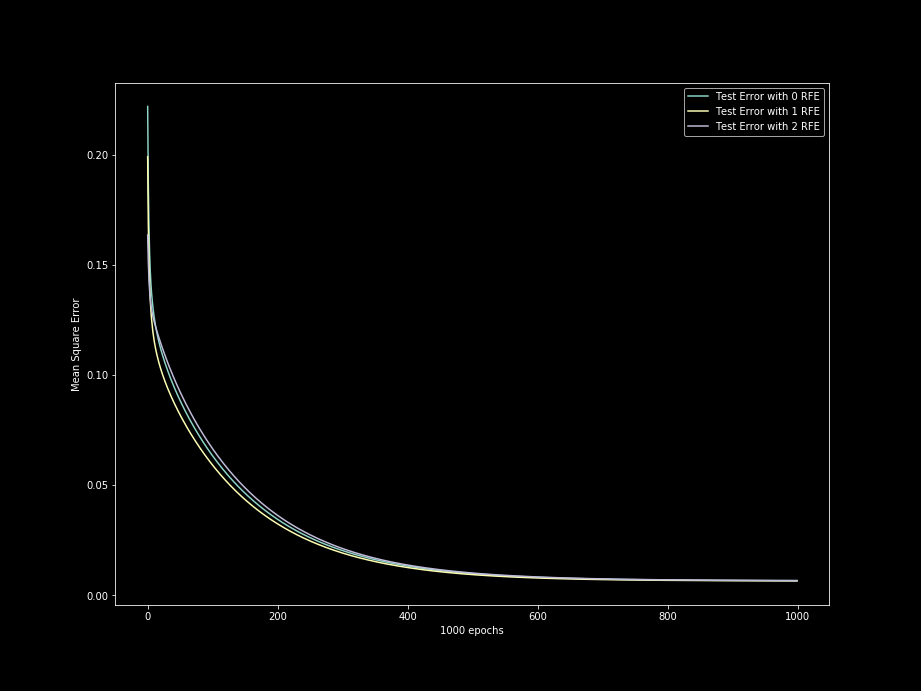
\includegraphics[width=0.8\linewidth]{assets/plots2/part3_7.png}
        \caption{Plot of accuracy predictions for different number of features removed by RFE}
        \label{fig:rfe3}
    \end{subfigure}
\end{figure}
\begin{figure}[H]
    \ContinuedFloat
    \begin{subfigure}{1\textwidth}
        \centering
        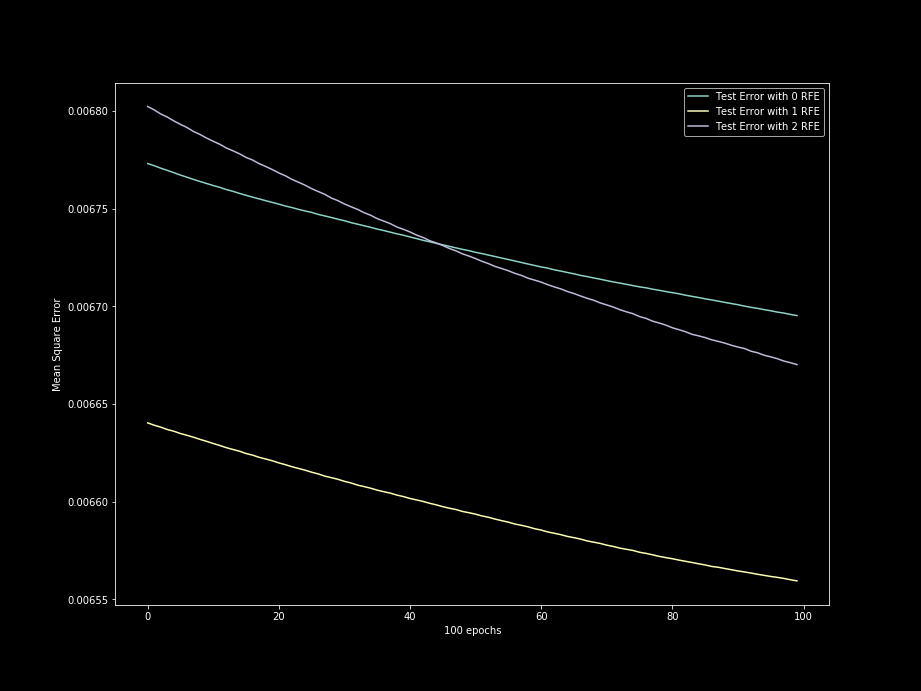
\includegraphics[width=0.8\linewidth]{assets/plots2/part3_8.png}
        \caption{Plot of accuracy predictions for different number of features removed by RFE - last 100 epochs}
        \label{fig:rfe3_zoom}
    \end{subfigure}
\end{figure}

As seen from Figure \ref{fig:rfe3_zoom}, the removal of just one feature (University Ranking) is the best for improving the model performance. The next iteration of RFE which removed SOP actually reduced the performance of the model to a level similar to when no RFE is performed. As such, the removal of just 1 feature is optimal in this case. A more detailed discussion will be discussed in the conclusion.

\subsection{Question 4}
\label{2q4}
\begin{quote}
4. Design a four-layer neural network and a five-layer neural network, with the hidden layers having 50 neurons each. Use a learning rate of $10^{-3}$ for all layers and optimal feature set selected in part (3). Introduce dropouts (with a keep probability of 0.8) to the layers and report the accuracies. Compare the performances of all the networks (with and without dropouts) with each other and with the 3-layer network.
\end{quote}
\begin{figure}[H]
    \begin{subfigure}{1\textwidth}
        \centering
        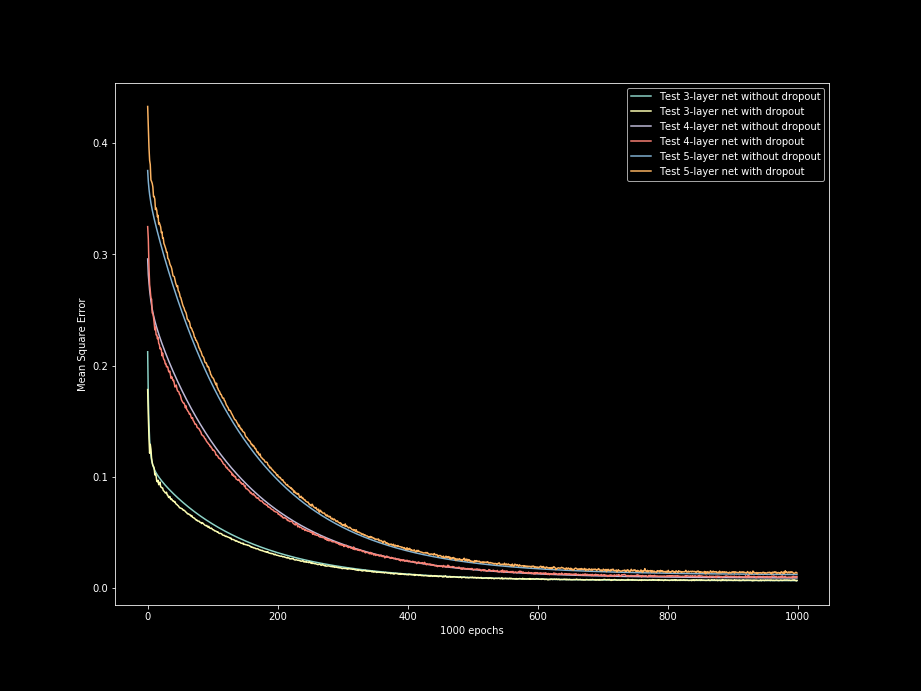
\includegraphics[width=0.8\linewidth]{assets/plots2/part4_1.png}
        \caption{Test errors for different network layers with and without dropout}
        \label{fig:2_4_1}
    \end{subfigure}
\end{figure}
\begin{figure}[H]
    \ContinuedFloat
    \begin{subfigure}{1\textwidth}
        \centering
        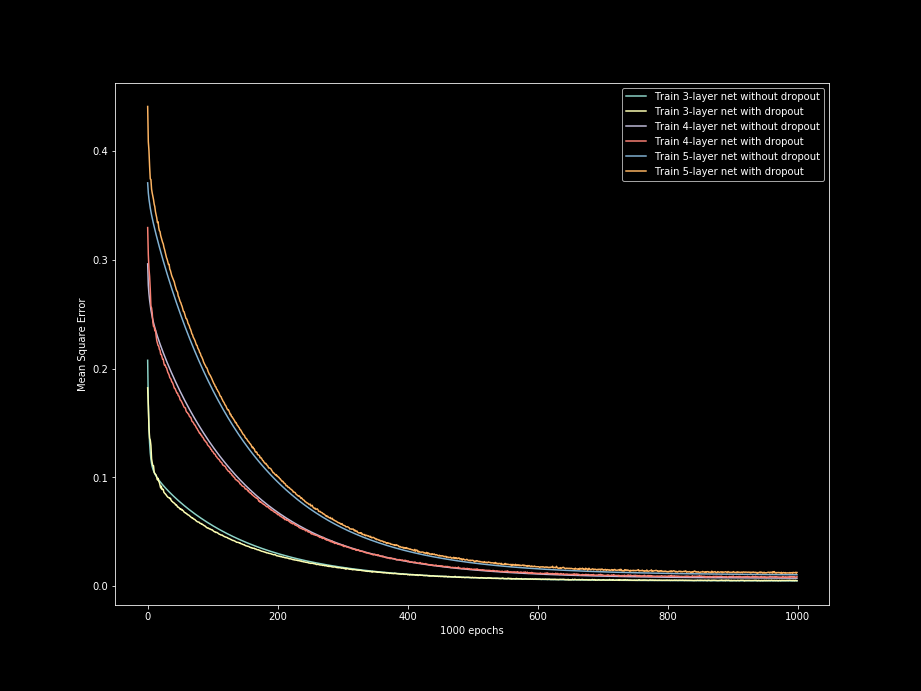
\includegraphics[width=0.8\linewidth]{assets/plots2/part4_2.png}
        \caption{Train errors for different network layers with and without dropout}
        \label{fig:2_4_2}
    \end{subfigure}
    \caption{Mean Square Errors for different network layers with and without dropout}
    \label{fig:2_4_3}
\end{figure}

From the results given in Figure \ref{fig:2_4_3}, for both \ref{fig:2_4_1} and \ref{fig:2_4_2}, we can see that the 3-layered network without dropout yields the least mean square error and it converges the fastest and yields the lowest mean square error, which means the best performance. Also, it has the least complexity by having only 3-layers, which reduces the tendency to overfit. For this dataset, a general trend can also be observed that as the number of layers increases, the mean square error and epoch to converge increases. The dropout reduces overfitting and thus improving the accuracy of the network itself, hence lower mean square error, better performance. Also generally, the introduction of dropouts will increase the performance of models in this regression dataset.

\newpage
\pagenumbering{roman}
% %%%% ADD BIBLOGARPHY
\printbibliography

\end{document}
